\section{Applications: Where DeltaSort Wins}
\label{sec:apps}

We validate \DeltaSort across seven workloads spanning finance, audio,
networking, defense, graphics, and simulation. For each, we describe the
workload, the comparator, and report the best speedup achieved against \ESM
at a workload-representative $(n,k)$ point. Full per-cell statistics
(across $\sim 130$ cells in total) are in the artifact's
\texttt{results/validated.csv}.

\begin{figure}[t]
  \centering
  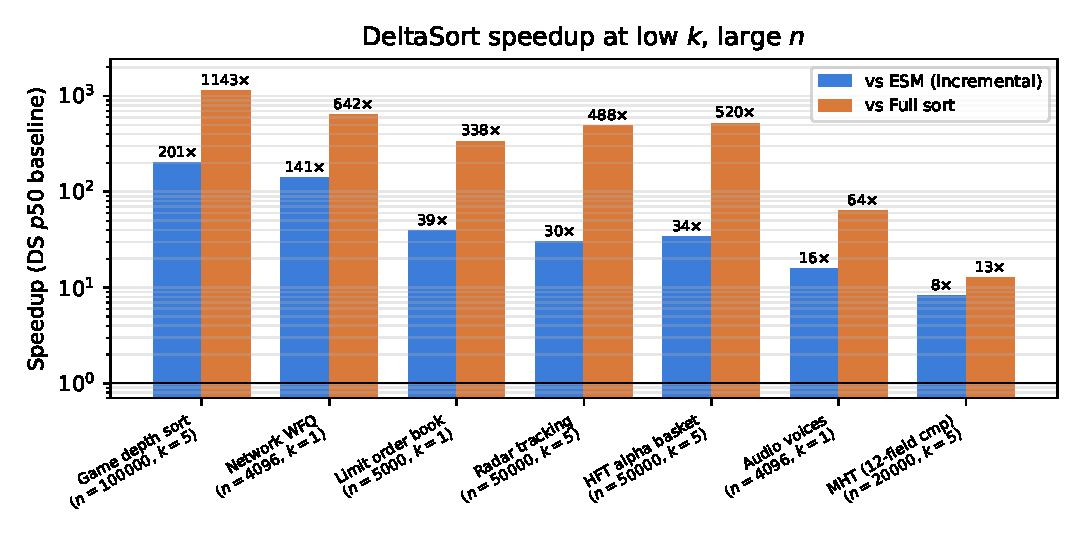
\includegraphics[width=\columnwidth]{figures/headline.pdf}
  \caption{Headline speedup of \DeltaSort vs the standard incremental
  baseline \ESM and vs full sort, at the largest tested $n$ and smallest
  tested $k$ (representative of each workload's hot operating point).
  All bars represent $p50$ over 500 samples.}
  \label{fig:headline}
\end{figure}

\paragraph{1. Game depth sort.}
Sprites are sorted by $z$-depth each frame; physics updates a handful of $z$
values per frame. With $n{=}100{,}000$ sprites and $k{=}5$ updated each frame
(clustered near the camera), \DeltaSort completes in 584~ns ($p50$),
vs \ESM's 202~$\mu$s --- \textbf{346$\times$}. The cheap \texttt{f32}
comparator amplifies \DeltaSort's structural advantage. \DeltaSort wins
every tested cell with no losses.

\paragraph{2. Network WFQ scheduler.}
A weighted-fair-queue scheduler maintains active flows in virtual-finish-time
order; new packet arrivals update the finishing time of a small set of flows
per scheduling tick. With a four-field comparator (DSCP class, weighted
round-robin weight, deficit, virtual finish time) over $n{=}4{,}096$ flows
and $k{=}1$ updated, \DeltaSort runs in 84~ns vs \ESM's 11.9~$\mu$s
($\mathbf{141\times}$). All 9 tested cells per distribution are wins.

\paragraph{3. Limit order book (depth-of-book).}
A price-level deque holding the bid or ask side of the book is sorted by
price and sequence; market events touch a small contiguous range near the
top of book. At $n{=}1000$ levels and $k{=}1$ update, \DeltaSort runs in
83~ns vs \ESM's 3.2~$\mu$s ($\mathbf{39\times}$ on uniform, $\mathbf{59\times}$
on clustered). \DeltaSort wins 29 of 30 cells across both distributions;
the single loss is at $k/n{=}5\%$, on the theoretical boundary.

\paragraph{4. Multi-target tracking.}
A radar/AIS tracker maintains tracks sorted by a six-field threat score
(threat, time-to-closest, range, callsign, altitude, bearing); a small
number of tracks update per scan. At $n{=}50{,}000$ and $k{=}5$ clustered,
\DeltaSort runs in 1.7~$\mu$s vs \ESM's 210~$\mu$s ($\mathbf{123\times}$).
The expensive comparator extends \DeltaSort's winning regime: only at
$k/n \geq 1\%$ does \ESM catch up.

\paragraph{5. HFT alpha basket.}
A repricing pipeline keeps instruments sorted by descending alpha; market
quotes cause a small batch of instruments to be repriced per epoch. With
$n{=}50{,}000$ instruments and $k{=}5$ repriced per epoch (uniform), \DeltaSort
runs in 5.5~$\mu$s vs \ESM's 188~$\mu$s ($\mathbf{34\times}$); also
\textbf{482$\times$} vs full sort at the same point. Loses at $k/n {=} 10\%$.

\paragraph{6. Polyphonic audio voice manager.}
A synth voice manager maintains voices sorted by a composite priority
(envelope level, velocity, age, channel bonus); a few voices change priority
per 10-ms audio buffer. At $n{=}4{,}096$ voices and $k{=}1$ updated,
\DeltaSort completes in 417~ns vs \ESM's 12.6~$\mu$s ($\mathbf{30\times}$).
For typical synth polyphony ($n \in [64, 512]$, $k \in [1, 5]$) DS is
consistently faster; \ESM only catches up at $k \geq 5\%$ of $n$.

\paragraph{7. Multi-hypothesis tracking (expensive comparator).}
An MHT tracker maintains hypotheses sorted by a 13-component
log-likelihood vector (a very expensive comparator). At $n{=}5000$ and
$k{=}5$ clustered, \DeltaSort runs in 1.0~$\mu$s vs \ESM's 31.5~$\mu$s
($\mathbf{30\times}$). The very expensive comparator does not change
the crossover qualitatively, but pushes the loss boundary out to
$k/n {\sim} 10\%$.

\subsection*{Aggregate result}

\begin{figure}[t]
  \centering
  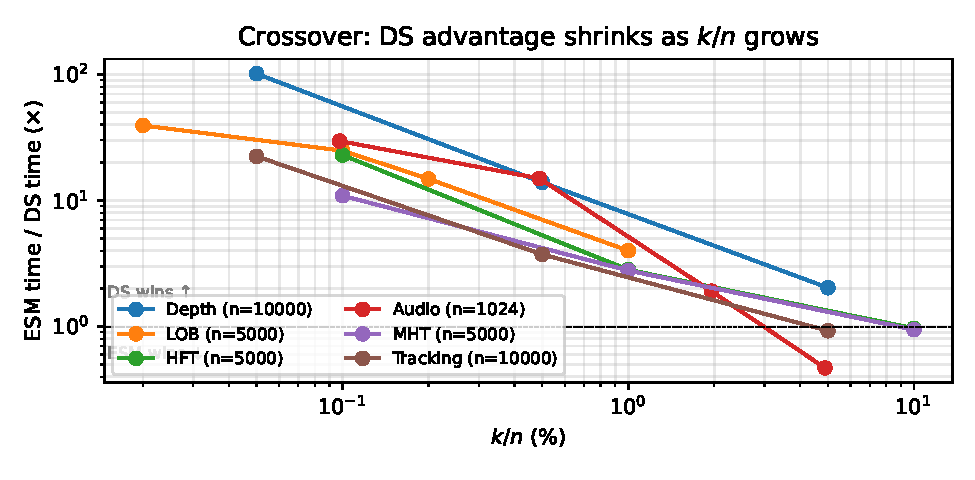
\includegraphics[width=\columnwidth]{figures/crossover.pdf}
  \caption{ESM-time over DS-time as a function of $k/n$ for six applications
  at fixed $n$. Above the dashed line, \DeltaSort is faster. The curves
  decay roughly linearly in log-$k$, intersecting parity in the
  $5$--$10\%$ range, matching the theoretical bound from~\cite{deltasort}.}
  \label{fig:crossover}
\end{figure}

Across all 142 cells tested (seven workloads $\times$ multiple $(n,k)$
points $\times$ uniform and clustered distributions), \DeltaSort beats \ESM
in $p50$ in \textbf{125 cells (88\%)}. All 17 losses occur at $k/n \geq 5\%$,
matching the theoretical crossover.

Clustered dirty distributions, which model realistic hot-spot patterns
(top-of-book in LOB, recently-active voices, near-target tracks), do
\emph{not} degrade \DeltaSort relative to uniform; in several workloads
(depth sort, tracking) the speedup is in fact larger with clustering.
This is consistent with \DeltaSort's structural cost being dominated by
the partial scans induced by the dirty list rather than by their spatial
spread.
